\documentclass[final,t]{beamer}
\mode<presentation>{ \usetheme{Major} }
\usepackage{times}
\usepackage{amsmath,amsthm, amssymb, latexsym}
\boldmath
\usepackage[english]{babel}

\usepackage{relsize}
\usepackage{multirow}
\usepackage{qtree}
\usepackage{stmaryrd}
\usepackage{booktabs}

%  \usepackage[font=small,format=plain,labelfont=bf,up,textfont=it,up]{caption}
\usepackage[font=normalsize,labelfont=small,bf,margin=2cm]{caption}
\usepackage[latin1]{inputenc}
\usepackage[orientation=landscape,size=a0,scale=1.6,debug]{beamerposter}
\usepackage{color,listings}
\usepackage{calc,xcolor}
\usepackage[absolute,overlay]{textpos}
\usepackage{smartdiagram}

\usepackage{wrapfig}

\usepackage[many]{tcolorbox}
\usepackage{tikz}
\usetikzlibrary{shadings}

\definecolor{lightblue}{rgb}{.85,.85,1} % 217 217 255
\definecolor{lightorange}{rgb}{1,.8,.6} % 255 204 153
\definecolor{lightgreen}{rgb}{.77,.91,.5} % 196 232 128
\definecolor{lightyellow}{rgb}{1,.98,.6} % 255 250 153
\definecolor{prussianblue}{rgb}{0.0,0.19,0.33}
\definecolor{gold}{rgb}{0.6,0.4,0.08}

\makeatletter
\pgfdeclarehorizontalshading{beamer@headfade}{5.4375ex+490pt}
{%
  color(0cm)=(lightblue);
  % color(15cm)=(lightblue);
  color(45cm)=(lightyellow);
  color(\paperwidth)=(gold)%
}
\addtoheadtemplate{\pgfuseshading{beamer@headfade}\vskip\dimexpr 0pt-52ex}{}
\makeatother


\newsavebox\CBox
\newenvironment{ColorBox}[3][black]{
    \par\noindent
    \def\borderColor{#1}\def\bgColor{#2}
    \begin{lrbox}{\CBox}
    \minipage{#3-2\fboxsep-2\fboxrule}
}{
    \endminipage\end{lrbox}%
    \fcolorbox{\borderColor}{\bgColor}{\usebox\CBox}\par
}

\lstset{language=java}
\lstset{breaklines=true}
\lstset{showstringspaces=false}
\lstset{tabsize=3}
\lstset{basicstyle=\ttfamily\scriptsize}
\lstset{breakautoindent=true}
\lstset{postbreak=\space}
%\lstset{commentstyle=\color{XcodeComments}}
%\lstset{keywordstyle=\color{XcodeKeywords}}
%\lstset{stringstyle=\color{XcodeStringstyle}}

%%%%%%%%%%%%%%%%%%%%%%%%%%%%%%%%%%%%%%%%%%%%%%%%%%%%%%%%%%%%%%%%%%%%%%%%%%%%%%%%%5
\title[]{Underwater Robotic Unit with Smart Sensing  \\ Technology
  for Water Quality Testing }
\author[Wright]{Elisia Wright, David Boughton and Dr. Janyl Jumadinova}
\institute{Department of Computer Science \\ Allegheny College, Meadville, PA}

%%%%%%%%%%%%%%%%%%%%%%%%%%%%%%%%%%%%%%%%%%%%%%%%%%%%%%%%%%%%%%%%%%%%%%%%%%%%%%%%%5
\begin{document}
    \begin{frame}{}
       % \vspace*{-6mm}
        \begin{columns}[t]
        	\begin{column}{1\linewidth}
            %%%%%%%%%%%%%%%%%%%%%%%%%%%%%%%%%%%%%%%%%%%%%%%%%%%%%%%%%%%%%%%%%%%%%
            %
            % Center column - Context
            %
            %%%%%%%%%%%%%%%%%%%%%%%%%%%%%%%%%%%%%%%%%%%%%%%%%%%%%%%%%%%%%%%%%%%%%

                %%%%%%%%%%%%%%%%%%%%%%%%%%%%%%%%%%%
                %
                % Project Objectives
                %
                %%%%%%%%%%%%%%%%%%%%%%%%%%%%%%%%%%%
                \begin{alertblock}{\textsc{\textbf{Project Objectives}}}
                    \vspace*{2mm}
                    The current methods for water quality testing either use a
                    single sensor to get a random sample for testing each water
                    quality	parameter separately, or data buoys that are able to
                    obtain readings from multiple sensors at a stationary location.
                    \vspace{2mm}

                    \emph{This project presents:}
                    \begin{itemize}
                        \item A single unit comprised of \textbf{multiple sensors}
                        that are able to collect data simultaneously for water
                        quality testing.
                        \item This multi-sensor unit attachable to the \textbf{underwater robot}
                        to collect data at various depths of the water column for
                        an extended period of time.
                        \item \textbf{Data collection} and \textbf{data analysis}
                        software to manage the data and assess certain trends in
                        the water quality over time.
                    \end{itemize}
                    \vspace*{6mm}
                \end{alertblock}
			\end{column}
		\end{columns}

		%%%%%%%%%%%%%%%%%%%%%%%%%%%%%%%%%%%%%%%%%%%%%%%%%%%%%%%%%%%%%%%%%%%%%
		\begin{columns}
		    %%%%%%%%%%%%%%%%%%%%%%%%%%%%%%%%%%%%%%%%%%%%%%%%%%%%%%%%%%%%%%%%%%%%%
            %
            % Left column - Context
            %
            %%%%%%%%%%%%%%%%%%%%%%%%%%%%%%%%%%%%%%%%%%%%%%%%%%%%%%%%%%%%%%%%%%%%%
            \begin{column}{.33\linewidth}
                %%%%%%%%%%%%%%%%%%%%%%%%%%%%%%%%%%%
                %
                % Method
                %
                %%%%%%%%%%%%%%%%%%%%%%%%%%%%%%%%%%%
                \begin{block}{\textsc{\textbf{Algal Blooms}}}
                  \vspace*{2mm}
                       
                  \begin{wrapfigure}{r}{0.5\textwidth}
                    \centering
                        \includegraphics[scale = 0.11]{assets/algalbloom.jpg}
                        \caption{Great Lakes: Oct. 2011}
                  \end{wrapfigure}
 Lake Erie algal blooms are an annual threat to the health
                       of \textbf{more than 11 million people}. Toxins produced
                       by harmful algal blooms  deeply affected the economy of the coastal towns
                       and the health of the environment and the public.
                       
                    \vspace*{2mm}
                \end{block}
                %%%%%%%%%%%%%%%%%%%%%%%%%%%%%%%%%%%
                %
                % Design
                %
                %%%%%%%%%%%%%%%%%%%%%%%%%%%%%%%%%%%
                \begin{alertblock}{\textsc{\textbf{System Design}}}
					   \begin{figure}
                    		\includegraphics[scale = 3.7]{assets/diagram.jpg}
                    	\caption{Different portions comprising the system}
                    	\end{figure}
                \end{alertblock}

            \end{column}
            %%%%%%%%%%%%%%%%%%%%%%%%%%%%%%%%%%%%%%%%%%%%%%%%%%%%%%%%%%%%%%%%%%%%%
            %
            % Center column 
            %
            %%%%%%%%%%%%%%%%%%%%%%%%%%%%%%%%%%%%%%%%%%%%%%%%%%%%%%%%%%%%%%%%%%%%%
            \begin{column}{.34\linewidth}
                 %%%%%%%%%%%%%%%%%%%%%%%%%%%%%%%%%%%
                %
                % Sensors
                %
                %%%%%%%%%%%%%%%%%%%%%%%%%%%%%%%%%%%
                \begin{alertblock}{\textsc{\textbf{Robotic and Sensor System}}}
                    \vspace*{2mm}

                   Our system includes a robotic unit, a collection of sensors, Arduino boards, and  programs.
                    \begin{itemize}
                    	%\item Sensors are all connected to an Arduino board
                      %for automatic data collection and analysis.
                    	\item A \textbf{waterproofed case} was designed to house sensors and boards on the robot.
						\item A remotely operated \textbf{robotic unit} was constructed with PVC pipe,
                      mesh, propellers, solder, and other materials, and is easily
                      deconstructable.
                     %	\item Waterproofed sensors on this robotic system allows for
                     % data to be collected for several hours at a time, which is
                     % then transmitted to the analytics software.
				 \end{itemize}
				
                    \begin{center}
                    \begin{figure}
                    \begin{tabular}{cc}
                    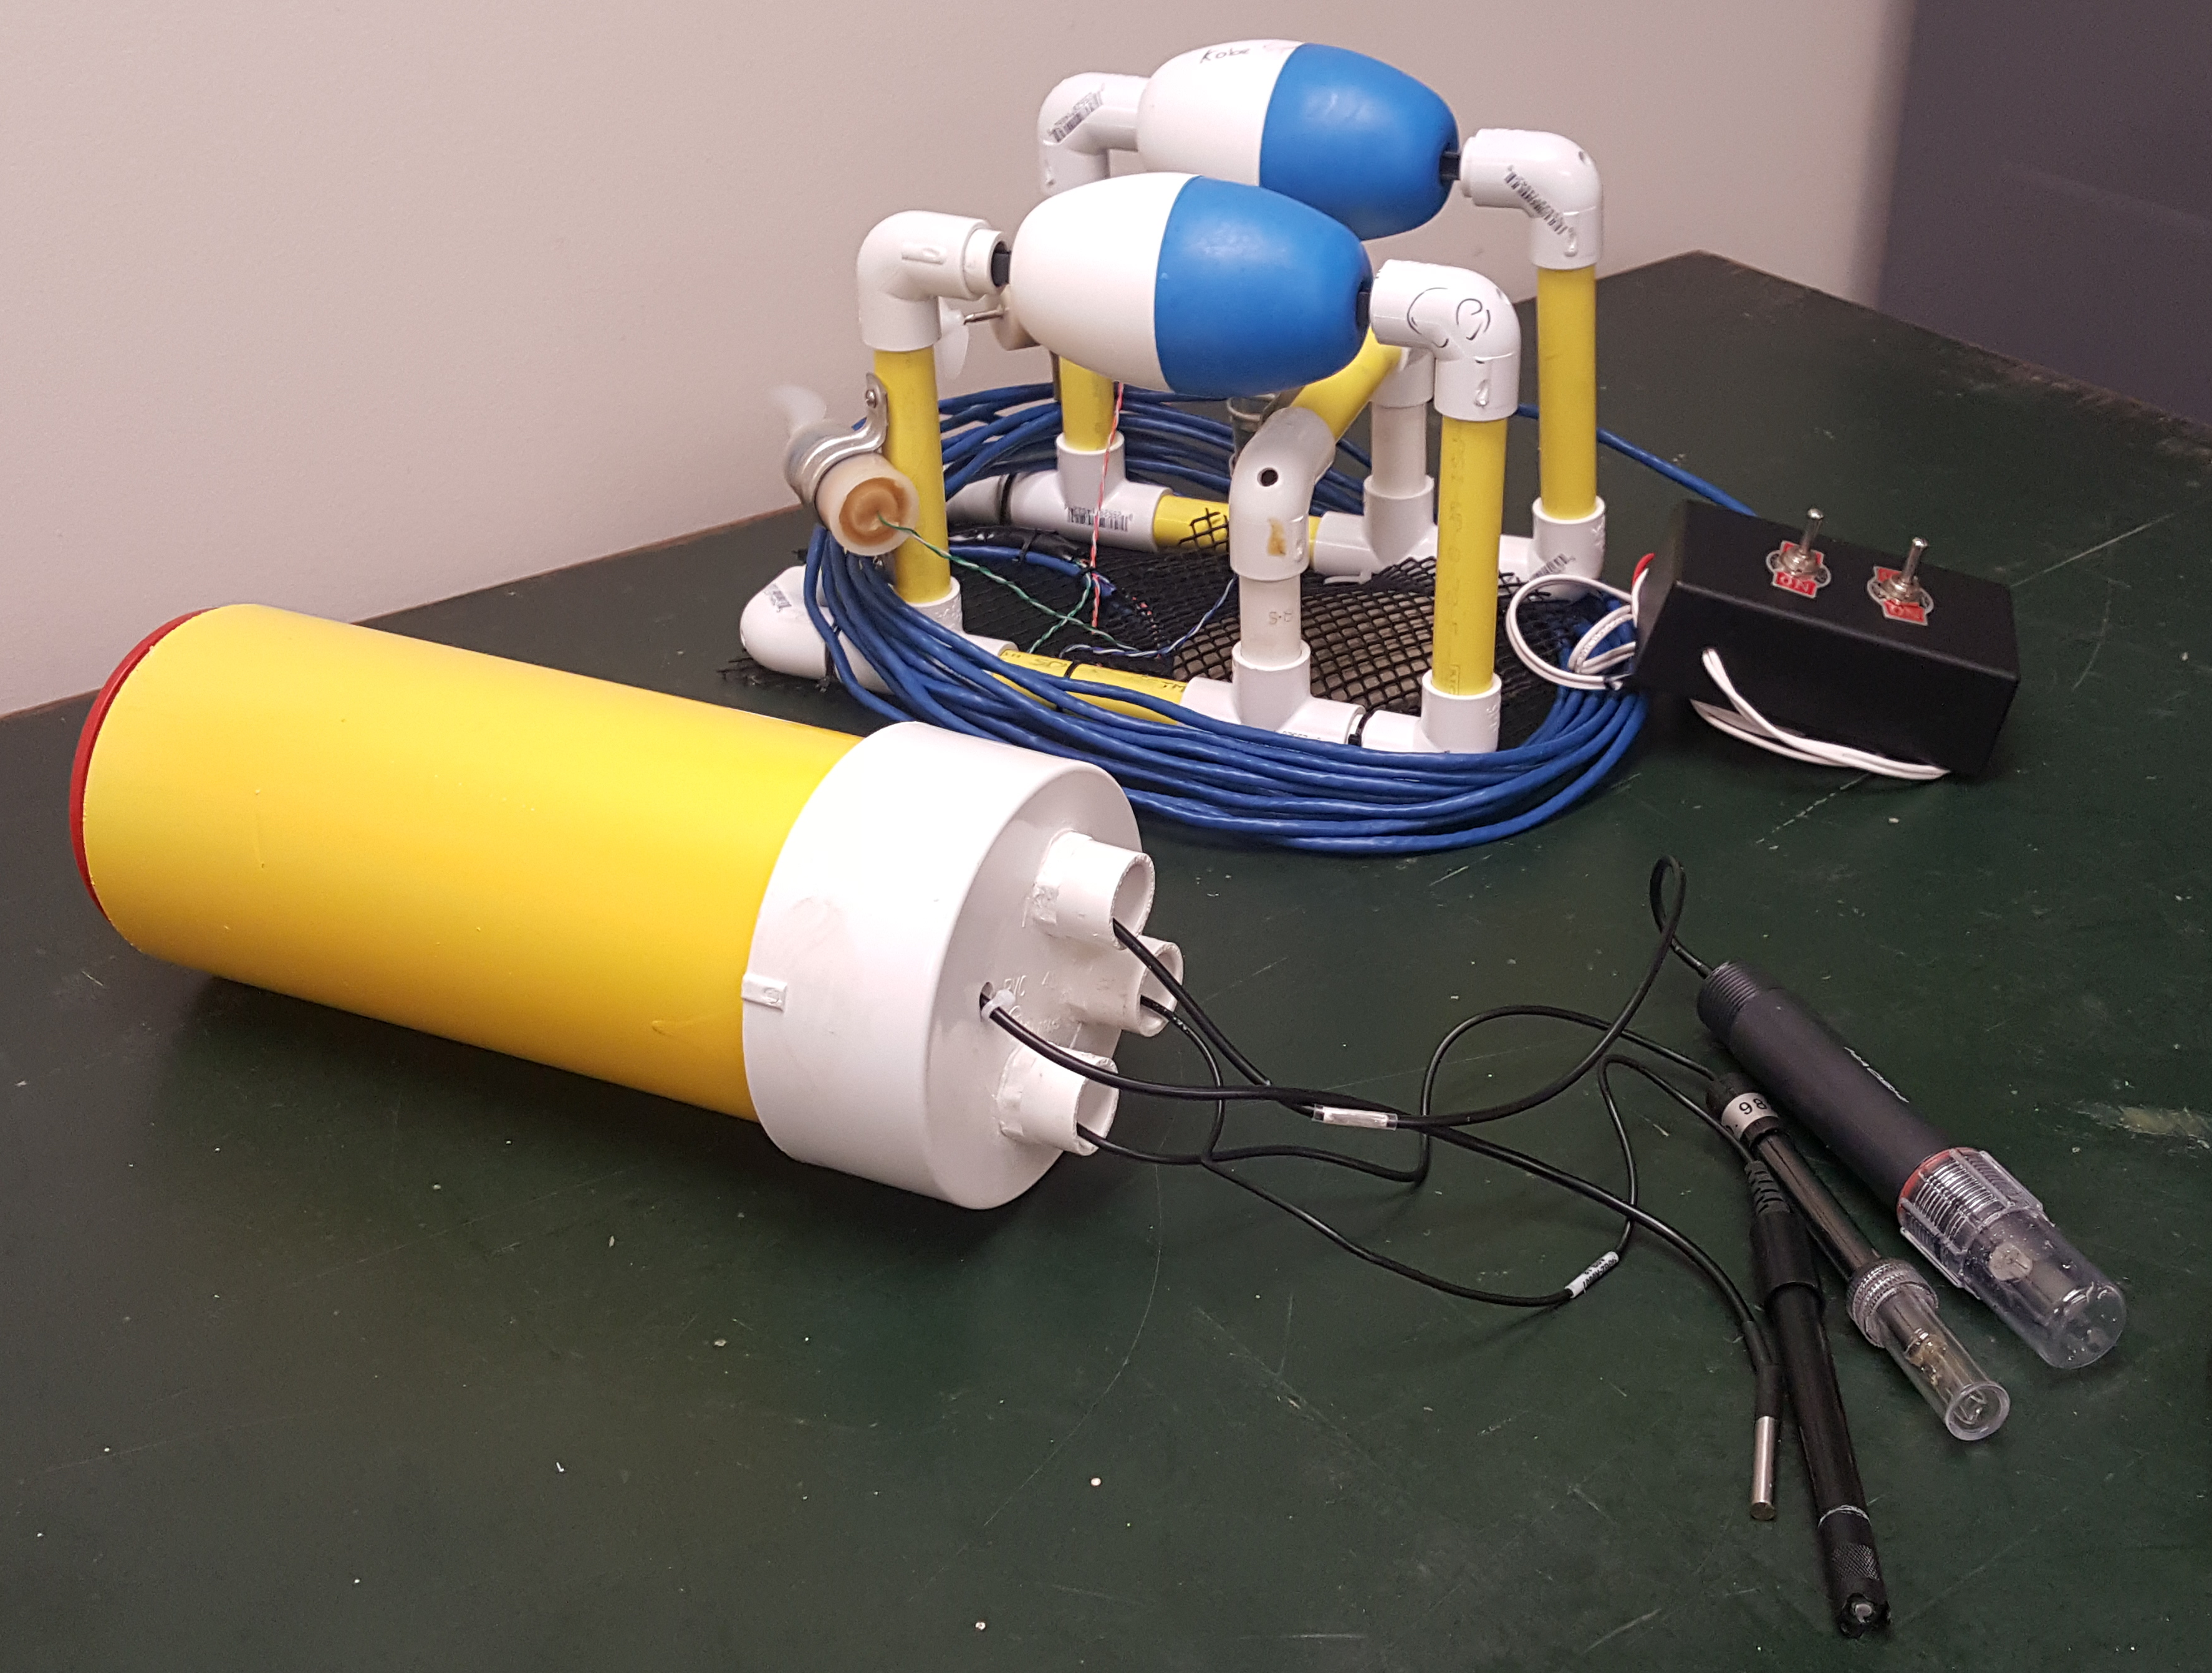
\includegraphics[scale = 0.16]{assets/robot1}
                    \hspace*{5mm}
                    &
                    \includegraphics[scale = 0.39]{assets/meworking1}
                    \end{tabular}
                    \caption{Detached system \hspace{30mm} Drilling holes for sensors}
                    \end{figure}
                    \end{center}

  				\end{alertblock}
  				
  				%%%%%%%%%%%%%%%%%%%%%%%%%%%%%%%%%%%
                %
                % Testing
                %
                %%%%%%%%%%%%%%%%%%%%%%%%%%%%%%%%%%%
                \begin{block}{\textsc{\textbf{Testing}}}
                    \vspace*{2mm}
                    %\begin{itemize}
                    	%\item 
                    	The robotic system was initially tested in the pool for buoyancy and general operation validation.
                    	%\item All sensors were calibrated and also tested individually.
                    	\vspace{-0.5in}
                    	\begin{center}
                    	\begin{tabular}{l|l}
                    	\textbf{Sensors} & \textbf{Testing Values} \\
                    	\hline 
                    	Temperature & 40F - 70F \\
                    	pH & Standard Buffer Solutions 4.0 and 7.0 \\
                    	Dissolved Oxygen & 0.5 mol/L NaOH Solution \\
                    								%&  (Sodium Hydroxide) \\
                    	Conductivity &  Buffer Solutions 1413us/cm and 12.88ms/cm 
                    	\end{tabular}
                    	\end{center}
                     %\end{itemize}

                   % \vspace*{3mm}
                \end{block}

            \end{column}
            %%%%%%%%%%%%%%%%%%%%%%%%%%%%%%%%%%%%%%%%%%%%%%%%%%%%%%%%%%%%%%%%%%%%%
            %
            % Right column - Outcomes
            %
            %%%%%%%%%%%%%%%%%%%%%%%%%%%%%%%%%%%%%%%%%%%%%%%%%%%%%%%%%%%%%%%%%%%%%
            \begin{column}{.33\linewidth}

                %%%%%%%%%%%%%%%%%%%%%%%%%%%%%%%%%%%
                %
                % Testing
                %
                %%%%%%%%%%%%%%%%%%%%%%%%%%%%%%%%%%%
                \begin{block}{\textsc{\textbf{Data Analysis}}}
                    \vspace*{-15mm}

                    \begin{center}
                    \begin{figure}
                    \begin{tabular}{cc}
                    \includegraphics[scale = 1.3]{assets/plot1}
                    \hspace*{-15mm}
                    &
                    \hspace*{-15mm}
                    \includegraphics[scale = 1.3]{assets/plot3}
                    \end{tabular}
                    \caption{Distribution  \hspace{80mm} Relationship \\ of the sensor data collected in Lake Erie}
                    \end{figure}
                    \end{center}
                    \begin{itemize}
                    	%\item Data analysis software was written in Python and includes machine learning algorithms to aggregate, learn and predict trends in the collected data.
                    	\item Statistical analysis of the collected data is first performed.
                    	\item Time series \textbf{forecasting} is used to predict future trends in the water quality.
                    	\item K-means \textbf{Clustering} is applied to learn relationships between water quality sensor measurements.   
                    \end{itemize}

                    \vspace*{3mm}
                \end{block}

                %%%%%%%%%%%%%%%%%%%%%%%%%%%%%%%%%%%
                %
                % Results
                %
                %%%%%%%%%%%%%%%%%%%%%%%%%%%%%%%%%%%
                \begin{alertblock}{\textsc{\textbf{Future Work}}}
                    \vspace*{3mm}
                    \begin{enumerate}
                    	\item Over a period of this summer, measurements from Lake Erie will be taken at
                      different levels of the water column.
                    	\item The results of this work, including collected data and its analysis will be shared with other researchers.
                      	\item Data analysis algorithms will be enhanced and automated with the data collection workflow.
                      	\item Autonomous robotic unit will be designed. 
                    	%\item The data retrieved can be used to protect coastal environments and surrounding communities.
                    \end{enumerate}

                    \vspace*{3mm}
                \end{alertblock}
            \end{column}

        \end{columns}
    \end{frame}
\end{document}
